% Fig 13: LCU circuit (TikZ redraw of the former yquant version), drawn in the
% style/palette of Figs 1, 4, 8: orange = state preparation (PREP), green =
% unitaries, violet = measurement. Filled dot = control on |1>, open = on |0>.
\begingroup
\definecolor{prepC}{RGB}{255,167,51}
\definecolor{uC}{RGB}{38,200,110}
\definecolor{mC}{RGB}{99,110,200}
\tikzset{
  qwire/.style={line width=0.6pt},
  prepg/.style={draw=prepC!60!black, line width=0.7pt, fill=prepC, rounded corners=2pt,
                minimum width=1.15cm, minimum height=1.2cm, inner sep=1.5pt},
  ug/.style={draw=uC!60!black, line width=0.7pt, fill=uC, rounded corners=2pt,
             minimum width=0.85cm, minimum height=1.2cm, inner sep=1.5pt},
  mtr/.style={draw=mC!60!black, line width=0.7pt, fill=mC, rounded corners=1pt,
              minimum width=0.6cm, minimum height=0.45cm, inner sep=1pt},
}
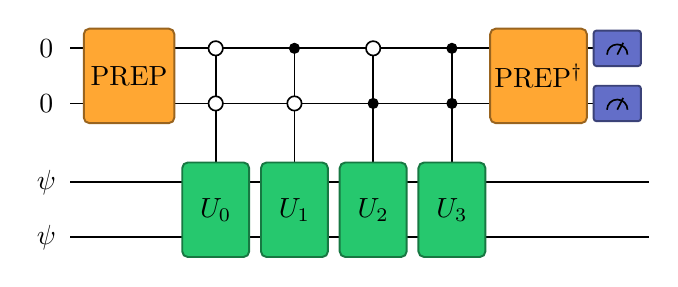
\begin{tikzpicture}[x=1cm,y=1cm, every node/.style={font=\rmfamily}]
% wires: two ancillas (top), two system qubits (bottom)
\foreach \y in {0,-0.7}{
  \node at (0.2,\y) {$\ket{0}$};
  \draw[qwire] (0.5,\y) -- (7.45,\y);
}
\foreach \y in {-1.7,-2.4}{
  \node at (0.2,\y) {$\ket{\psi}$};
  \draw[qwire] (0.5,\y) -- (7.85,\y);
}
% control lines (drawn first, controls and boxes go on top)
\foreach \x in {2.35,3.35,4.35,5.35}{
  \draw[qwire] (\x,0) -- (\x,-1.45);
}
% PREP on the ancillas
\node[prepg] at (1.25,-0.35) {PREP};
% SELECT: U_i on the system, controlled on the ancilla state |i>
\node[ug] at (2.35,-2.05) {$U_0$};
\node[ug] at (3.35,-2.05) {$U_1$};
\node[ug] at (4.35,-2.05) {$U_2$};
\node[ug] at (5.35,-2.05) {$U_3$};
% controls: open circle = condition on |0>, filled dot = condition on |1>
% U_0 fires on |00>, U_1 on |01> (a0=1), U_2 on |10> (a1=1), U_3 on |11>
\foreach \x in {2.35,4.35}{ \draw[qwire, fill=white] (\x,0) circle (2.6pt); }
\foreach \x in {3.35,5.35}{ \filldraw (\x,0) circle (1.8pt); }
\foreach \x in {2.35,3.35}{ \draw[qwire, fill=white] (\x,-0.7) circle (2.6pt); }
\foreach \x in {4.35,5.35}{ \filldraw (\x,-0.7) circle (1.8pt); }
% PREP^dagger on the ancillas
\node[prepg] at (6.45,-0.35) {PREP$^{\dagger}$};
% measure ancillas; post-select on the all-zeros outcome
\foreach \y in {0,-0.7}{
  \node[mtr] at (7.45,\y) {};
  \draw[black, line width=0.6pt] (7.32,\y-0.08) arc[start angle=180, end angle=0, radius=0.13];
  \draw[black, line width=0.6pt] (7.45,\y-0.08) -- (7.525,\y+0.07);
}
\end{tikzpicture}%
\endgroup
